\chapter{Microscope Basics}
\thispagestyle{fancy}
\fancyhead[RE,LO]{Technical Document \thechapter}
\label{chap:scope-basic}

\section*{Microscope Parts}
Below is a list of the different parts of the microscope and their function.
If you are having trouble identifying a particular part, or are unsure of how to operate something, ask your TA for assistance.

\begin{figure}[ht]
	\centering
	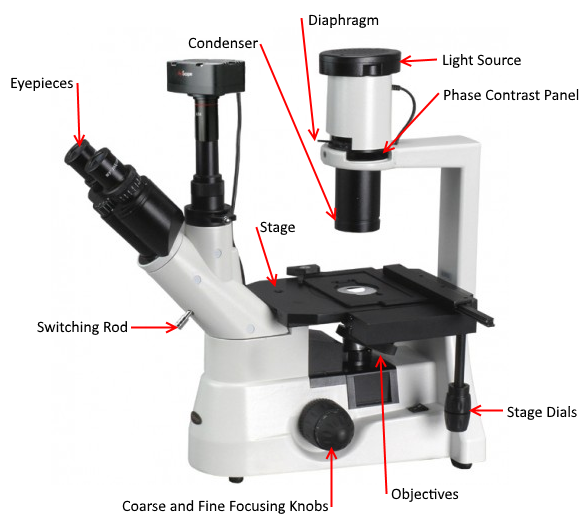
\includegraphics[scale=0.7]{microscope.png}
	\caption{Diagram of the microscope parts.}
	\label{fig:microscope}
\end{figure}

\begin{itemize}
\setlength\itemsep{1pt}
\item Eyepieces
\begin{itemize}
	\setlength\itemsep{1pt}
	\item Adjustable to fit both eyes. If eyelashes obstruct view, move closer to the eyepieces.
%	\item Sometimes easier if one eye is closed
\end{itemize}
\item Light Source, Condenser, Phase Contrast Panel
\begin{itemize}
	\setlength\itemsep{1pt}
	\item Condenser concentrates light from illumination source.
	\item Phase rings in front of the light source allow the microscope to translate phase shifts in light that goes through a transparent sample into brightness changes in the observed images. This allows for very useful imaging of transparent samples that would be difficult with standard bright field imaging.
	\item The light intensity can be controlled by adjusting the orange wheel on the bottom left of the machine.
\end{itemize}
\item Diaphragm
\begin{itemize}
	\setlength\itemsep{1pt}
	\item Lever controls an iris, allowing the user to control the amount of light hitting the sample. Very often, higher detail can be observed by allowing less light through the iris.
\end{itemize}
\item Stage
\begin{itemize}
	\setlength\itemsep{1pt}
	\item Place the sample on the microscope stage carefully. The stage can be moved relative to the objectives using the dials below the stage to the right. Align the sample directly over the objective, so the light is shining directly on the sample.
\end{itemize}
\item Objectives
\begin{itemize}
	\setlength\itemsep{1pt}
	\item Objectives collect the light from the samples and focus it to form an image in the eyepiece or CCD camera. Rotating turret holds four different objective lenses: 4X, 10X, 20X, and 40X. Always start with a low magnification objective: find, center, then focus on the sample before moving on to a higher magnification.
%	\item Always lower objectives using the coarse adjustment knob before rotating the turret.
\end{itemize}
\item Coarse and Fine Focusing Knobs
\begin{itemize}
	\item Bring sample into view using the coarse adjustment knob (inner knob). Once sample is in view, use the fine adjustment knob (outer knob) to achieve the sharpest possible image. Be careful when using the coarse adjustment knob, hitting the slide with the objective can scratch the objective or crack the slide.
\end{itemize}
\item CCD Camera
\begin{itemize}
	\setlength\itemsep{1pt}
	\item Adjust the switching rod to go from eyepiece-only to dual-view mode. Camera can be rotated using the adjustable pin below the lens
\end{itemize}
\end{itemize}

\newpage

\section*{Microscope Software}
The capture software for the microscope is called ``Amscope'', it should be located on the desktop.
The software has a viewing area in the center and adjustment settings on the left.
To begin, click `MU503' under `Camera List' to see the view from the camera in the viewing area.
Then adjust the following settings:
\begin{itemize}
\item Set the `Live' and `Snap' resolutions. While capturing video it's best to use `1280 x 960'.
\item Uncheck `Auto Exposure'. Adjust the `Exposure Time' to approximately 33 ms, this means you will be capturing video at 30 fps. Turn the Gain down to 1.0, increase this if you cannot get a bright enough image.
\item In `Color Adjustment', reduce Saturation to 0 and Contrast to 100. Adjust the brightness as necessary.
\end{itemize}
\paragraph*{To capture a video:}
See figure \ref{fig:am-cap} while following along with the steps below:
\begin{itemize}
\item Click the `Record' button on the left, this will open a window called `Video file'.
\item Type the name of the video file that you want to capture; select your group's data folder as the save location. Click Next
\item select the `avi' format, click Next.
\item Under `Encoder' setect `None Compressor', leave the encode parameter quality set at 100. Click Next.
\item Check the box next to `Time Limit', then input the number of seconds that you want to capture video. Clicking `Finish' (or pressing Enter) will begin the video capture.
\end{itemize}
The microscope can be very sensitive to table vibrations, especially when you are imaging at high magnifications. 
After setting all the video capture parameters, wait a bit before starting the capture for the vibrations to die down.
While the camera is capturing, do your best to not disturb the table.

\paragraph*{To capture a `low fps' video:}
Occasionally we may need to capture video at a low frame rate over a long period of time.
To do this, we will set the software to capture an image every few seconds (see figure \ref{fig:low-fps}).
Then, we will use ImageJ to stitch the images together into a .avi video.
\begin{itemize}
\item Navigate to `Capture $>$ Start Time-lapse (Auto Capture)...'
\item In the window that opens, begin by setting the directory where you want all the images to be saved. It's advised that you create a new folder where you will save all the images, as this will make the rest of the steps easier.
\item Under File, set `Name Format' to `nnnn (sequence)', in `File Prefix' input the names that you want given to the videos, set `File Type' to png.
\item Under Capture Mode, select `Time Slot' and input the number of seconds between each frame.
\item Check `Total Images', then input the number of frames that you want captured.
\item Clicking OK or pressing Enter will begin the time-lapse. As before, wait for the vibrations to die down before beginning the capture, and avoid touching the table.
\item After the time-lapse is complete, open ImageJ and navigate to `File $>$ Import $>$ Image Sequence...'.
\item Navigate to the folder where your time-lapse images are saved, choose any of the images and click Open.
\item In the Sequence Options window, make sure `Sort names numerically' is checked, then click OK.
\item After processing the images, a new window will open. Navigate to `File $>$ Save As $>$ AVI...'. Set Compression to `Uncompressed', set Frame Rate to 25, click OK. Enter the file name, then press Save.
\item After creating the avi file, delete the time-lapse images to avoid using unnecessary space.
\end{itemize}

\begin{figure}[ht]
	\centering
	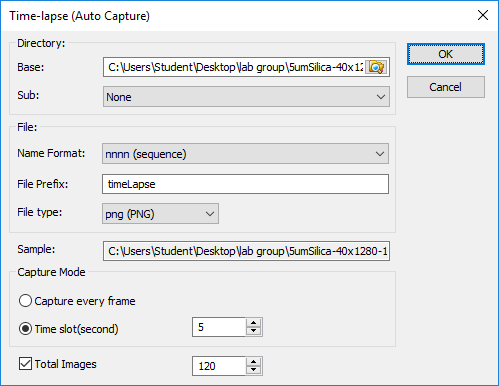
\includegraphics[width=0.7\textwidth]{amscope06}
	\caption{Amscope `low fps' video capturing settings.}
	\label{fig:low-fps}
\end{figure}

\begin{figure}[ht]
	\centering
	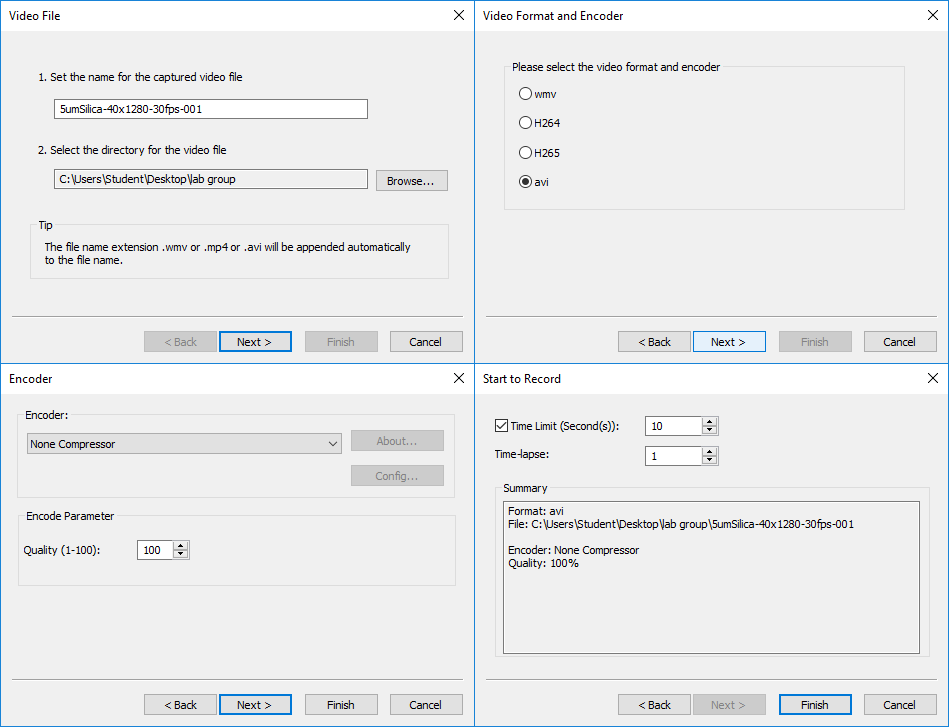
\includegraphics[width=\textwidth]{amscope08}
	\caption{Amscope video capturing settings.}
	\label{fig:am-cap}
\end{figure}


%\section*{Eyepieces:}
%\begin{itemize}
%	\setlength\itemsep{1pt}
%	\item Adjustable to fit both eyes
%	\item Sometimes easier if one eye is closed
%	\item If eyelashes obstruct view, move closer to the eyepieces
%\end{itemize}
%
%\section*{Light Source, Condenser, Phase Contrast Panel:}
%\begin{itemize}
%	\setlength\itemsep{1pt}
%	\item Condenser concentrates light from illumination source
%	\item Phase rings in front of the light source allow the microscope to translate phase shifts in light that goes through a transparent sample into brightness changes in the observed images. This allows for very useful imaging of transparent samples that would be difficult with standard bright field imaging.
%	\item The light intensity can be controlled by adjusting the orange wheel on the bottom left of the machine.
%\end{itemize}
%
%\section*{Diaphragm:}
%\begin{itemize}
%	\setlength\itemsep{1pt}
%	\item Lever controls an iris, allowing the user to control the amount of light hitting the sample
%	\item Very often, higher detail can be observed by allowing less light through the iris
%\end{itemize}
%
%\section*{Stage:}
%\begin{itemize}
%	\setlength\itemsep{1pt}
%	\item Place the sample slide on the microscope stage carefully
%	\item The stage can be moved relative to the objectives using the dials below the stage to the right
%	\item Align the sample directly over the objective, so the light is shining directly on the sample
%\end{itemize}
%
%\section*{Objectives:}
%\begin{itemize}
%	\setlength\itemsep{1pt}
%	\item Objectives collect the light from the samples and focus it to form an image in the eyepiece or CCD camera.
%	\item Rotating turret holds four different objective lenses: 4X, 10X, 20X, and 40X
%	\item Always start with a low magnification objective: find, center and focus on the sample before moving on to a higher magnification.
%	\item Always lower objectives using the coarse adjustment knob before rotating the turret
%\end{itemize}
%
%\section*{Coarse and Fine Focusing Knobs:}
%\begin{itemize}
%	\setlength\itemsep{1pt}
%	\item Bring sample into view using the coarse adjustment knob (inner knob)
%	\item Once sample is in view, use the fine adjustment knob (outer knob) to achieve the sharpest possible image.
%	\item Be careful when using the coarse adjustment knob, hitting the slide with the objective can scratch the objective or crack the slide.
%\end{itemize}
%
%\section*{CCD Camera:}
%\begin{itemize}
%	\setlength\itemsep{1pt}	
%	\item Camera can be rotated using the adjustable pin below the lens
%\end{itemize}